\documentclass[10pt,a4paper]{article}

% =========================================================
% PACKAGES
% =========================================================

\usepackage[T1]{fontenc}
\usepackage[utf8]{inputenc}
\usepackage[british]{babel}

\usepackage[
    top=10mm,
    bottom=10mm,
    left=11mm,
    right=11mm
]{geometry}

\usepackage{graphicx}
\usepackage{xcolor}
\usepackage{enumitem}
\usepackage{multicol}
\usepackage{titlesec}
\usepackage{microtype}
\usepackage{hyperref}
\usepackage{fontawesome5}
\usepackage{FiraSans}

\renewcommand{\familydefault}{\sfdefault}

% =========================================================
% COLORS
% =========================================================

\definecolor{navy}{HTML}{243B5A}
\definecolor{blue}{HTML}{2F527F}
\definecolor{lightblue}{HTML}{EEF3F8}
\definecolor{darkgray}{HTML}{333333}
\definecolor{gray}{HTML}{666666}

% =========================================================
% HYPERLINKS
% =========================================================

% Normal hyperlinks throughout the CV
\hypersetup{
    colorlinks=true,
    urlcolor=black,
    linkcolor=black,
    pdfborder={0 0 0}
}

% Header-only hyperlinks
\newcommand{\headerhref}[2]{%
    \begingroup
    \hypersetup{
        colorlinks=true,
        urlcolor=white,
        linkcolor=white
    }%
    \href{#1}{#2}%
    \endgroup
}

% =========================================================
% PAGE
% =========================================================

\pagestyle{empty}

\setlength{\parindent}{0pt}
\setlength{\parskip}{0pt}

% =========================================================
% MULTICOLUMN
% =========================================================

\setlength{\columnsep}{7mm}

% =========================================================
% LISTS
% =========================================================

\setlist[itemize]{
    leftmargin=4.5mm,
    itemsep=1.5pt,
    topsep=2pt,
    parsep=0pt,
    partopsep=0pt
}

% =========================================================
% SECTION STYLE
% =========================================================

\titleformat{\section}
    {\large\bfseries\color{navy}}
    {}
    {0pt}
    {}
    [\vspace{1pt}\color{navy}\titlerule]

\titlespacing*{\section}
    {0pt}
    {7pt}
    {4pt}

% =========================================================
% CUSTOM COMMANDS
% =========================================================

\newcommand{\job}[4]{
    \textbf{\large #1}
    \hfill
    \textbf{\small #4}

    \textit{#2} --- #3

    \vspace{1mm}
}

\newcommand{\project}[2]{
    \textbf{#1}\\
    \textit{\small #2}
}

\newcommand{\skill}[2]{
    \textbf{#1:} #2
    \par\vspace{1.2mm}
}

% =========================================================
% DOCUMENT
% =========================================================

\begin{document}

% =========================================================
% HEADER
% =========================================================

\colorbox{navy}{
\begin{minipage}{0.97\textwidth}

\color{white}

\begin{minipage}[c]{0.72\textwidth}

\vspace{5mm}

{\Huge\bfseries SHAH ABDUL MAZID}

\vspace{1mm}

{\Large\bfseries AI/ML ENGINEER}

\vspace{2mm}

Generative AI
\quad|\quad
LLMs
\quad|\quad
RAG
\quad|\quad
Computer Vision
\quad|\quad
NLP

\vspace{3mm}

\small

\faMapMarker* \ Dhaka, Bangladesh
\quad
\faEnvelope\ 
\headerhref{
    mailto:shahabdulmazid.ezan@yahoo.com
}{
    shahabdulmazid.ezan@yahoo.com
}

\vspace{1mm}

\faPhone* \ +880 1531329222
\quad
\faLinkedin\ 
\headerhref{
    https://www.linkedin.com/in/shahabdulmazid
}{
    LinkedIn
}
\quad
\faGithub\ 
\headerhref{
    https://github.com/Shah-Abdul-Mazid
}{
    GitHub
}
\quad
\faGraduationCap\
\headerhref{
    https://scholar.google.com/citations?user=TYkiwUgAAAAJ
}{
    Google Scholar
}

\vspace{5mm}

\end{minipage}
\hfill
\begin{minipage}[c]{0.19\textwidth}

\vspace{3mm}

\begin{flushright}

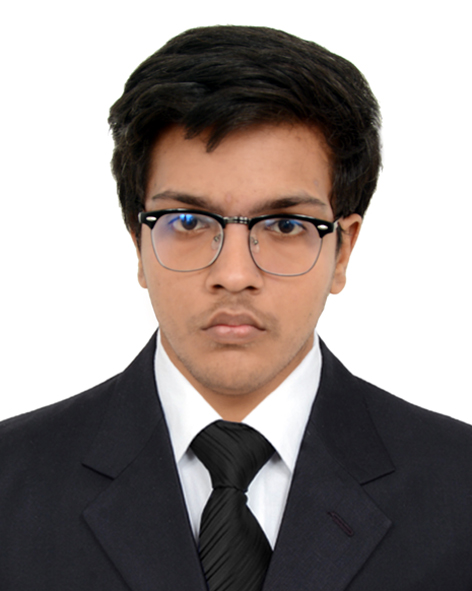
\includegraphics[
    width=29mm,
    height=35mm,
    keepaspectratio
]{FD=109767.jpg}

\end{flushright}

\vspace{3mm}

\end{minipage}

\end{minipage}
}
\vspace{4mm}

% =========================================================
% PROFESSIONAL SUMMARY
% =========================================================

\section*{Professional Summary}

AI/ML Engineer with a B.Sc. in Computer Science and Engineering from East West University, majoring in Intelligent Systems and Data Science. Experienced in Generative AI, LLMs, RAG, Machine Learning, Deep Learning, Computer Vision, and NLP. Skilled in building AI applications using Python, PyTorch, TensorFlow, FastAPI, Pinecone, OpenAI APIs, and AWS. Passionate about AI research and developing intelligent solutions for real-world problems.

\vspace{2mm}

% =========================================================
% TWO COLUMNS
% =========================================================

\begin{multicols}{2}

% =========================================================
% COLUMN 1
% =========================================================

\section{Technical Skills}

\skill{Languages}{
Python, Java, C/C++, JavaScript, TypeScript, SQL
}

\skill{AI / ML}{
Machine Learning, Deep Learning, Transfer Learning,
Model Evaluation, Data Preprocessing
}

\skill{Generative AI}{
Generative AI, LLMs, RAG, Prompt Engineering,
AI Agents, Agentic AI, Multi-Agent Systems
}

\skill{NLP}{
Natural Language Processing, Semantic Search,
Vector Search, Embeddings, Sentence Transformers,
Document Q\&A, AI Chatbots
}

\skill{Computer Vision}{
Object Detection, Image Classification,
Medical Imaging, YOLO, OpenCV,
Grad-CAM, CBAM Attention
}

\skill{Frameworks}{
PyTorch, TensorFlow, Keras, Scikit-learn,
NumPy, Pandas, Matplotlib, Plotly
}

\skill{Backend}{
FastAPI, REST APIs, JWT Authentication,
API Integration, PDF Processing
}

\skill{Frontend}{
React, Next.js, Streamlit, Gradio
}

\skill{Databases}{
Pinecone, Vector Databases, MongoDB,
MySQL, SQLite
}

\skill{Cloud / DevOps}{
AWS, EC2, Docker, PM2, Git, GitHub
}

\skill{Automation}{
n8n, Workflow Automation, API Integration
}

% =========================================================
% EDUCATION
% =========================================================

\section{Education}

\textbf{B.Sc. in Computer Science \& Engineering}

\textit{East West University}

\hfill
\textbf{2021--2026}

Major: Intelligent Systems \& Data Science

\vspace{2mm}

\textbf{Higher Secondary Certificate}

\textit{Dhaka Ideal College}

\hfill
\textbf{2018--2020}

Science

\vspace{2mm}

\textbf{Secondary School Certificate}

\textit{Badshah Faisal Institute}

\hfill
\textbf{2016--2018}

Science

% =========================================================
% LANGUAGES
% =========================================================

\section{Languages}

\textbf{Bengali} --- Native

\vspace{1mm}

\textbf{English} --- Professional Working Proficiency

% =========================================================
% RESEARCH INTERESTS
% =========================================================

\section{Research Interests}

\begin{itemize}

\item Generative AI and Large Language Models

\item Retrieval-Augmented Generation

\item Multi-Agent AI Systems

\item Healthcare AI

\item Computer Vision and Medical Imaging

\item Natural Language Processing

\item Intelligent Recommendation Systems

\item Model Interpretability

\end{itemize}

% =========================================================
% CAREER FOCUS
% =========================================================

\section{Career Focus}

AI/ML Engineering

\vspace{1mm}

Generative AI

\vspace{1mm}

LLM and RAG Systems

\vspace{1mm}

AI Research

\vspace{1mm}

Computer Vision

\vspace{1mm}

Data Science

% =========================================================
% COLUMN 2
% =========================================================
\section{Tools \& Platforms}
\skill{Models \& APIs}{
OpenAI API, Llama 2, Mistral, Claude API, HuggingFace Models
}

\skill{Vector DBs \& Search}{
Pinecone, Weaviate, Milvus, Chroma, FAISS
}

\skill{Deployment}{
Hugging Face Hub, AWS SageMaker, Docker Hub, Streamlit Cloud
}

\skill{Dev Tools}{
VS Code, Git, GitHub, Jupyter, Google Colab, Linux/Ubuntu
}

\skill{APIs \& Integrations}{
OpenAI API, Google Maps, Stripe, Google Sheets, Anthropic API
}

\section{Key Achievements}

\begin{itemize}
\item Published research on interpretable ML for agricultural disease diagnosis (ICCIT 2025)
\item Built enterprise RAG platform processing 10,000+ documents with 95\%+ accuracy
\item Developed traffic detection system for real-world Bangladesh traffic conditions
\item Designed multi-agent AI system handling complex enterprise workflows
\item 9+ IBM and AWS certifications in AI/ML specializations
\end{itemize}
\newpage
\section{Professional Highlights}

\textbf{Published Researcher:} MangoStack ensemble model published in ICCIT 2025

\vspace{1mm}

\textbf{RAG Specialist:} Built enterprise platforms for document-based Q\&A systems

\vspace{1mm}

\textbf{Full-Stack AI:} End-to-end ML systems from training to production deployment

\vspace{1mm}

\textbf{Automation Expert:} n8n workflow automation for business process efficiency

% =========================================================
% EXPERIENCE
% =========================================================
\section{Professional Experience}

\job
{AI Engineer}
{Neuroxyte}
{Narayanganj, Dhaka Division, Bangladesh}
{July 2026 -- Current}

\begin{itemize}

\item Develop and deploy AI solutions using Generative AI, LLMs, RAG, and intelligent automation.

\item Build AI applications and scalable backend services using Python and FastAPI.

\item Design LLM-based workflows, conversational AI systems, and retrieval-augmented applications.

\item Integrate AI models, external APIs, and third-party services to deliver reliable end-to-end solutions.

\end{itemize}

\vspace{2mm}

\job
{AI Engineer}
{Softvence Agency}
{Dhaka, Bangladesh}
{Feb 2026 -- July 2026}

\begin{itemize}

\item Developed RAG-based chatbots using Large Language Models for intelligent question answering.

\item Built FastAPI backend services and integrated AI models and external APIs.

\item Developed Text-to-Speech and voice generation systems for interactive AI applications.

\item Automated business workflows using n8n and implemented Generative AI and RAG solutions.

\end{itemize}

\vspace{2mm}

\section{Selected Projects}

% ---------------------------------------------------------

\project
{Nexus Intelligence}
{Enterprise Multi-Agent AI Platform}

\vspace{0.5mm}

Built a full-stack enterprise AI platform for secure Q\&A across private documents, spreadsheets, and web data.

\begin{itemize}
\item Implemented RAG, multi-agent routing, Pinecone retrieval, feedback memory, JWT authentication, and PII detection.
\item \textbf{Tech:} FastAPI, Next.js, React, TypeScript, OpenAI, Pinecone, AWS.
\end{itemize}

\vspace{1.5mm}

% ---------------------------------------------------------

\project
{HR Policies RAG Chatbot}
{AI-Powered Document Q\&A}

\vspace{0.5mm}

Built a citation-aware chatbot that answers HR policy questions from organizational PDF documents using RAG.

\begin{itemize}
\item Implemented PDF processing, semantic search, vector retrieval, and LLM-based response generation.
\item \textbf{Tech:} Python, FastAPI, Streamlit, Pinecone, Llama 2, Sentence Transformers.
\end{itemize}

\vspace{1.5mm}

% ---------------------------------------------------------

\project
{Bangladesh Traffic Flow Dataset}
{Deep Learning Vehicle Detection}

\vspace{0.5mm}

Developed a computer vision system for vehicle detection and classification under Bangladesh traffic conditions.

\begin{itemize}
\item Implemented YOLO detection with Grad-CAM/EigenCAM-based model interpretation and interactive inference.
\item \textbf{Tech:} PyTorch, YOLO, OpenCV, NumPy, Pandas, Streamlit, Gradio.
\end{itemize}

\vspace{1.5mm}

% ---------------------------------------------------------

\project
{Brain Tumor Detection and Classification}
{MobDenseNet with CBAM Attention}

\vspace{0.5mm}

Developed a hybrid MobileNetV2--DenseNet121 model with CBAM attention for MRI-based brain tumor classification.

\begin{itemize}
\item Applied preprocessing, augmentation, classification, and Grad-CAM for explainable predictions.
\item \textbf{Tech:} PyTorch, MobileNetV2, DenseNet121, CBAM, Grad-CAM, Streamlit.
\end{itemize}

\vspace{1.5mm}

% ---------------------------------------------------------

\project
{WhatsUpIn}
{AI-Powered Travel Recommendation Engine}

\vspace{0.5mm}

Built an AI travel platform that generates personalized itineraries and automates travel-related workflows.

\begin{itemize}
\item Integrated OpenAI, n8n, Google Maps, Google Sheets, and Stripe for end-to-end automation.
\item \textbf{Tech:} OpenAI, n8n, APIs, Google Maps, Google Sheets, Stripe.
\end{itemize}
% =========================================================
% PUBLICATION
% =========================================================
\section{Publication}

\textbf{MangoStack: A Lightweight, Interpretable Ensemble for Real-Time Mango Leaf Disease Diagnosis}\\
\textbf{Authors:} Raiyan Gani, Yusuf Salehin, Md. Shakil Bhuiyan, 
\textbf{Shah Abdul Mazid}, Monisha Bani Nibedita Shuci, Shamim Ripon\\[-0.5mm]
\textit{2025 28th International Conference on Computer and Information Technology (ICCIT), IEEE}, 
pp.~2235--2240.\\[-1mm]
DOI: \href{https://doi.org/10.1109/ICCIT68739.2025.11490181}
{10.1109/ICCIT68739.2025.11490181}

\vspace{1mm}

\textbf{Uncertainty-Aware Chest Pathology Detection with Vision and Language Transformers}\\
\textbf{Authors:} \textbf{Shah Abdul Mazid}, Monisha Bani Nibedita Shuci, 
Mahia Mehrun Safa, Md. Ashikur Rahman Anik, Md. Omor Faruk Sejan, 
Khandhakar Shatu Moni, Md. Sazzad Hossain, Md. Adnan Morshed, Ahmed Wasif Reza\\[-0.5mm]
\textit{Innovations in Data Analytics}, Springer Nature, 2026, 
pp.~397--417.\\[-1mm]
DOI: \href{https://doi.org/10.1007/978-3-032-27845-6_34}
{10.1007/978-3-032-27845-6\_34}


% =========================================================
% CERTIFICATIONS
% =========================================================

\section{Certifications}

\begin{itemize}

\item IBM Deep Learning with PyTorch, Keras and TensorFlow

\item DeepLearning.AI TensorFlow Developer

\item IBM Machine Learning

\item IBM RAG and Agentic AI

\item Building AI Agents and Agentic Workflows

\item IBM AI Developer

\item AWS Generative AI and AI Agents with Amazon Bedrock

\item IBM AI Engineering

\item IBM Data Science

\end{itemize}

% =========================================================
% COMPETITIONS
% =========================================================

\section{Competitions \& Awards}

\textbf{Network War} --- EWU Telecommunication Club, 2024

\vspace{1mm}

\textbf{IT Olympiad} --- CSE FEST, East West University, 2024

\vspace{1mm}

\textbf{In House Programming Battle} --- EWUCoPC, 2022

% =========================================================
% ONLINE PROFILES
% =========================================================

\section{Online Profiles}

\textbf{Portfolio:}
\href{https://shah-abdul-mazid-portfolio.vercel.app/home}
{Portfolio Profile}

\vspace{0.5mm}

\textbf{GitHub:}
\href{https://github.com/Shah-Abdul-Mazid}
{Github Profile}

\vspace{0.5mm}

\textbf{LinkedIn:}
\href{https://www.linkedin.com/in/shahabdulmazid}
{LinkedIn Profile}

\vspace{0.5mm}

\textbf{Nexus Intelligence:}
\href{https://ai-rag-project-llm-based.vercel.app/auth/login}
{Live Demo}

\end{multicols}

\end{document}